% Options for packages loaded elsewhere
\PassOptionsToPackage{unicode}{hyperref}
\PassOptionsToPackage{hyphens}{url}
%
\documentclass[
]{book}
\usepackage{amsmath,amssymb}
\usepackage{lmodern}
\usepackage{iftex}
\ifPDFTeX
  \usepackage[T1]{fontenc}
  \usepackage[utf8]{inputenc}
  \usepackage{textcomp} % provide euro and other symbols
\else % if luatex or xetex
  \usepackage{unicode-math}
  \defaultfontfeatures{Scale=MatchLowercase}
  \defaultfontfeatures[\rmfamily]{Ligatures=TeX,Scale=1}
\fi
% Use upquote if available, for straight quotes in verbatim environments
\IfFileExists{upquote.sty}{\usepackage{upquote}}{}
\IfFileExists{microtype.sty}{% use microtype if available
  \usepackage[]{microtype}
  \UseMicrotypeSet[protrusion]{basicmath} % disable protrusion for tt fonts
}{}
\makeatletter
\@ifundefined{KOMAClassName}{% if non-KOMA class
  \IfFileExists{parskip.sty}{%
    \usepackage{parskip}
  }{% else
    \setlength{\parindent}{0pt}
    \setlength{\parskip}{6pt plus 2pt minus 1pt}}
}{% if KOMA class
  \KOMAoptions{parskip=half}}
\makeatother
\usepackage{xcolor}
\IfFileExists{xurl.sty}{\usepackage{xurl}}{} % add URL line breaks if available
\IfFileExists{bookmark.sty}{\usepackage{bookmark}}{\usepackage{hyperref}}
\hypersetup{
  pdftitle={Aula 5},
  pdfauthor={Pedro Leite},
  hidelinks,
  pdfcreator={LaTeX via pandoc}}
\urlstyle{same} % disable monospaced font for URLs
\usepackage{color}
\usepackage{fancyvrb}
\newcommand{\VerbBar}{|}
\newcommand{\VERB}{\Verb[commandchars=\\\{\}]}
\DefineVerbatimEnvironment{Highlighting}{Verbatim}{commandchars=\\\{\}}
% Add ',fontsize=\small' for more characters per line
\usepackage{framed}
\definecolor{shadecolor}{RGB}{248,248,248}
\newenvironment{Shaded}{\begin{snugshade}}{\end{snugshade}}
\newcommand{\AlertTok}[1]{\textcolor[rgb]{0.94,0.16,0.16}{#1}}
\newcommand{\AnnotationTok}[1]{\textcolor[rgb]{0.56,0.35,0.01}{\textbf{\textit{#1}}}}
\newcommand{\AttributeTok}[1]{\textcolor[rgb]{0.77,0.63,0.00}{#1}}
\newcommand{\BaseNTok}[1]{\textcolor[rgb]{0.00,0.00,0.81}{#1}}
\newcommand{\BuiltInTok}[1]{#1}
\newcommand{\CharTok}[1]{\textcolor[rgb]{0.31,0.60,0.02}{#1}}
\newcommand{\CommentTok}[1]{\textcolor[rgb]{0.56,0.35,0.01}{\textit{#1}}}
\newcommand{\CommentVarTok}[1]{\textcolor[rgb]{0.56,0.35,0.01}{\textbf{\textit{#1}}}}
\newcommand{\ConstantTok}[1]{\textcolor[rgb]{0.00,0.00,0.00}{#1}}
\newcommand{\ControlFlowTok}[1]{\textcolor[rgb]{0.13,0.29,0.53}{\textbf{#1}}}
\newcommand{\DataTypeTok}[1]{\textcolor[rgb]{0.13,0.29,0.53}{#1}}
\newcommand{\DecValTok}[1]{\textcolor[rgb]{0.00,0.00,0.81}{#1}}
\newcommand{\DocumentationTok}[1]{\textcolor[rgb]{0.56,0.35,0.01}{\textbf{\textit{#1}}}}
\newcommand{\ErrorTok}[1]{\textcolor[rgb]{0.64,0.00,0.00}{\textbf{#1}}}
\newcommand{\ExtensionTok}[1]{#1}
\newcommand{\FloatTok}[1]{\textcolor[rgb]{0.00,0.00,0.81}{#1}}
\newcommand{\FunctionTok}[1]{\textcolor[rgb]{0.00,0.00,0.00}{#1}}
\newcommand{\ImportTok}[1]{#1}
\newcommand{\InformationTok}[1]{\textcolor[rgb]{0.56,0.35,0.01}{\textbf{\textit{#1}}}}
\newcommand{\KeywordTok}[1]{\textcolor[rgb]{0.13,0.29,0.53}{\textbf{#1}}}
\newcommand{\NormalTok}[1]{#1}
\newcommand{\OperatorTok}[1]{\textcolor[rgb]{0.81,0.36,0.00}{\textbf{#1}}}
\newcommand{\OtherTok}[1]{\textcolor[rgb]{0.56,0.35,0.01}{#1}}
\newcommand{\PreprocessorTok}[1]{\textcolor[rgb]{0.56,0.35,0.01}{\textit{#1}}}
\newcommand{\RegionMarkerTok}[1]{#1}
\newcommand{\SpecialCharTok}[1]{\textcolor[rgb]{0.00,0.00,0.00}{#1}}
\newcommand{\SpecialStringTok}[1]{\textcolor[rgb]{0.31,0.60,0.02}{#1}}
\newcommand{\StringTok}[1]{\textcolor[rgb]{0.31,0.60,0.02}{#1}}
\newcommand{\VariableTok}[1]{\textcolor[rgb]{0.00,0.00,0.00}{#1}}
\newcommand{\VerbatimStringTok}[1]{\textcolor[rgb]{0.31,0.60,0.02}{#1}}
\newcommand{\WarningTok}[1]{\textcolor[rgb]{0.56,0.35,0.01}{\textbf{\textit{#1}}}}
\usepackage{longtable,booktabs,array}
\usepackage{calc} % for calculating minipage widths
% Correct order of tables after \paragraph or \subparagraph
\usepackage{etoolbox}
\makeatletter
\patchcmd\longtable{\par}{\if@noskipsec\mbox{}\fi\par}{}{}
\makeatother
% Allow footnotes in longtable head/foot
\IfFileExists{footnotehyper.sty}{\usepackage{footnotehyper}}{\usepackage{footnote}}
\makesavenoteenv{longtable}
\usepackage{graphicx}
\makeatletter
\def\maxwidth{\ifdim\Gin@nat@width>\linewidth\linewidth\else\Gin@nat@width\fi}
\def\maxheight{\ifdim\Gin@nat@height>\textheight\textheight\else\Gin@nat@height\fi}
\makeatother
% Scale images if necessary, so that they will not overflow the page
% margins by default, and it is still possible to overwrite the defaults
% using explicit options in \includegraphics[width, height, ...]{}
\setkeys{Gin}{width=\maxwidth,height=\maxheight,keepaspectratio}
% Set default figure placement to htbp
\makeatletter
\def\fps@figure{htbp}
\makeatother
\setlength{\emergencystretch}{3em} % prevent overfull lines
\providecommand{\tightlist}{%
  \setlength{\itemsep}{0pt}\setlength{\parskip}{0pt}}
\setcounter{secnumdepth}{5}
\usepackage{booktabs}
\ifLuaTeX
  \usepackage{selnolig}  % disable illegal ligatures
\fi
\usepackage[]{natbib}
\bibliographystyle{plainnat}

\title{Aula 5}
\author{Pedro Leite}
\date{2022-07-18}

\begin{document}
\maketitle

{
\setcounter{tocdepth}{1}
\tableofcontents
}
\hypertarget{pipes}{%
\chapter{Pipes}\label{pipes}}

\begin{center}
\includegraphics[width=3.77in]{figuras/ceci_pipe} \end{center}

\hypertarget{origem-do-pipe}{%
\section{Origem do Pipe}\label{origem-do-pipe}}

O conceito de \emph{pipe} existe pelo menos desde os anos 1970, quando Douglas McIlroy originalmente propôs os pipelines no Unix. O operador tinha o objetivo de simplificar comandos cujos resultados deveriam ser passados para outros comandos.

Por essa descrição já conseguimos ter uma ideia de onde vem o seu nome: pipe em inglês significa ``cano'', referindo-se ao transporte das saídas dos comandos. Em portugês o termo é traduzido como ``canalização'' ou ``encadeamento'', mas no dia-a-dia é mais comum usar o termo em inglês.

A partir daí o pipe tem aparecido nas mais diversas aplicações, desde HTML até o R. Ele pode ter várias aparências, mas o seu objetivo é sempre o mesmo: transportar resultados.

No R o pipe tem um símbolo um pouco estranho (\%\textgreater\%), mas no fundo ele não passa de uma função infixa, ou seja, uma função que aparece entre os seus argumentos (como a + b ou a \%in\% b). Na verdade é por isso mesmo que ele tem porcentagens antes e depois: porque no R uma função infixa só pode ser declarada assim, entre parêntesis.

\hypertarget{pacote-magrittr}{%
\section{Pacote magrittr}\label{pacote-magrittr}}

\begin{center}
\includegraphics[width=1.09in]{figuras/logo} \end{center}

O pacote \emph{magrittr} fornece um conjunto de operadores que tornam seu código mais fácil de ler.

Por quê?

\begin{itemize}
\tightlist
\item
  Cria sequências estruturais de operações (pipelines ou ``encanamentos'') da esquerda para a direita (em vez de dentro pra fora);
\item
  evita chamar funções aninhadas;
\item
  minimiza a necessidade de variáveis locais e definição de funções;
\item
  torna mais fácil adicionar etapas em qualquer local da sequência de operações.
\end{itemize}

Os pipes conectam os valores da esquerda em expressões que aparecem do lado direito, i.e.~podemos substituir \texttt{f(x)} com \texttt{x\ \%\textgreater{}\%\ f()}, onde \texttt{\%\textgreater{}\%} é o operador pipe.

Vamos começar demonstrando sua funcionalidade básica. Carregue o pacote magrittr e declare o pipe usando Ctrl + Shift + M.

\begin{Shaded}
\begin{Highlighting}[]
\FunctionTok{library}\NormalTok{(magrittr)}
\NormalTok{mais\_tres }\OtherTok{\textless{}{-}} \ControlFlowTok{function}\NormalTok{(x) \{ x }\SpecialCharTok{+} \DecValTok{3}\NormalTok{ \}}
\NormalTok{sobre\_dois }\OtherTok{\textless{}{-}} \ControlFlowTok{function}\NormalTok{(x) \{ x }\SpecialCharTok{/} \DecValTok{2}\NormalTok{ \}}
\NormalTok{x }\OtherTok{\textless{}{-}} \DecValTok{1}\SpecialCharTok{:}\DecValTok{3}

\FunctionTok{sobre\_dois}\NormalTok{(}\FunctionTok{mais\_tres}\NormalTok{(x))}
\end{Highlighting}
\end{Shaded}

\begin{verbatim}
## [1] 2.0 2.5 3.0
\end{verbatim}

Perceba como fica difícil de entender o que está acontecendo primeiro? A linha
relevante começa com a divisão por 2, depois vem a soma com 3 e, por fim, os
valores de entrada.

É muito mais legível quando as funções são exibidas na ordem em que serão aplicadas.

Isso pode ser realizado se tivermos uma função que passa o resultado do que
está à sua esquerda para a função que está à sua direita:

\begin{Shaded}
\begin{Highlighting}[]
\NormalTok{x }\SpecialCharTok{\%\textgreater{}\%} \FunctionTok{mais\_tres}\NormalTok{() }\SpecialCharTok{\%\textgreater{}\%} \FunctionTok{sobre\_dois}\NormalTok{()}
\end{Highlighting}
\end{Shaded}

Ao juntar diversas funções com o pipe, o benefício torna-se mais aparente.
Considere o exemplo abaixo:

\begin{Shaded}
\begin{Highlighting}[]
\NormalTok{clima }\SpecialCharTok{\%\textgreater{}\%}
  \FunctionTok{filter}\NormalTok{(origem }\SpecialCharTok{\%in\%} \StringTok{\textquotesingle{}JFK\textquotesingle{}}\NormalTok{) }\SpecialCharTok{\%\textgreater{}\%}
  \FunctionTok{mutate}\NormalTok{(}\AttributeTok{temp\_celsius =}\NormalTok{ (temperatura }\SpecialCharTok{{-}} \DecValTok{32}\NormalTok{) }\SpecialCharTok{*} \DecValTok{5}\SpecialCharTok{/}\DecValTok{9}\NormalTok{) }\SpecialCharTok{\%\textgreater{}\%}
  \FunctionTok{head}\NormalTok{(}\DecValTok{5}\NormalTok{)}
\end{Highlighting}
\end{Shaded}

\begin{verbatim}
## # A tibble: 5 x 16
##   origem   ano   mes   dia  hora temperatura ponto_condensacao umidade
##   <chr>  <int> <int> <int> <int>       <dbl>             <dbl>   <dbl>
## 1 JFK     2013     1     1     1        39.0              26.1    59.4
## 2 JFK     2013     1     1     2        39.0              26.1    59.4
## 3 JFK     2013     1     1     3        39.9              27.0    59.5
## 4 JFK     2013     1     1     4        39.9              28.0    62.2
## 5 JFK     2013     1     1     5        39.0              27.0    61.6
## # ... with 8 more variables: direcao_vento <dbl>, velocidade_vento <dbl>,
## #   velocidade_rajada <dbl>, precipitacao <dbl>, pressao <dbl>,
## #   visibilidade <dbl>, data_hora <dttm>, temp_celsius <dbl>
\end{verbatim}

Quatro operações são realizadas para chegar ao conjunto de dados desejado, e
elas são escritas em uma ordem natural: a mesma ordem de sua execução. Além
disso, nenhuma variável temporária é necessária. Se necessitarmos de mais
uma operação, é fácil incluí-la na sequência de operações, em qualquer local
necessário.

\hypertarget{antes-do-pipe}{%
\section{Antes do pipe}\label{antes-do-pipe}}

Como as pessoas escreviam seus códigos antes do pipe?

Usando o pacote \texttt{pinguins}, calcule a média da massa corporal dos pinguins da
espécie ``Pinguim-de-adélia'' em diferentes ilhas.

Primeiro, vamos ler nossa base e visualizá-la:

\begin{Shaded}
\begin{Highlighting}[]
\NormalTok{pinguins}
\end{Highlighting}
\end{Shaded}

\begin{verbatim}
## # A tibble: 344 x 8
##    especie           ilha     comprimento_bico profundidade_bi~ comprimento_nad~
##    <fct>             <fct>               <dbl>            <dbl>            <int>
##  1 Pinguim-de-adélia Torgers~             39.1             18.7              181
##  2 Pinguim-de-adélia Torgers~             39.5             17.4              186
##  3 Pinguim-de-adélia Torgers~             40.3             18                195
##  4 Pinguim-de-adélia Torgers~             NA               NA                 NA
##  5 Pinguim-de-adélia Torgers~             36.7             19.3              193
##  6 Pinguim-de-adélia Torgers~             39.3             20.6              190
##  7 Pinguim-de-adélia Torgers~             38.9             17.8              181
##  8 Pinguim-de-adélia Torgers~             39.2             19.6              195
##  9 Pinguim-de-adélia Torgers~             34.1             18.1              193
## 10 Pinguim-de-adélia Torgers~             42               20.2              190
## # ... with 334 more rows, and 3 more variables: massa_corporal <int>,
## #   sexo <fct>, ano <int>
\end{verbatim}

Podemos decompor nosso problema em uma séria de etapas:

\begin{itemize}
\tightlist
\item
  Filtrar pinguins para manter as observações da espécia ``Adélia''.
\item
  Agrupar os pinguins filtrados por ilha.
\item
  Sumarizar os pinguins agrupados e filtrados calculando a média da massa
  corporal.
\end{itemize}

Mas como implementamos esse código?

\hypertarget{etapas-intermediuxe1rias}{%
\subsection{Etapas intermediárias}\label{etapas-intermediuxe1rias}}

Uma opção é salvar cada etapa como um novo objeto:

\begin{Shaded}
\begin{Highlighting}[]
\NormalTok{pinguins\_1 }\OtherTok{\textless{}{-}} \FunctionTok{filter}\NormalTok{(pinguins, especie }\SpecialCharTok{\%in\%} \StringTok{"Pinguim{-}de{-}adélia"}\NormalTok{)}
\NormalTok{pinguins\_2 }\OtherTok{\textless{}{-}} \FunctionTok{group\_by}\NormalTok{(pinguins\_1, ilha)}
\NormalTok{(pinguins\_3 }\OtherTok{\textless{}{-}} \FunctionTok{summarise}\NormalTok{(pinguins\_2, }\AttributeTok{media\_mc =} \FunctionTok{mean}\NormalTok{(massa\_corporal, }\AttributeTok{na.rm =} \ConstantTok{TRUE}\NormalTok{)))}
\end{Highlighting}
\end{Shaded}

\begin{verbatim}
## # A tibble: 3 x 2
##   ilha      media_mc
##   <fct>        <dbl>
## 1 Biscoe       3710.
## 2 Dream        3688.
## 3 Torgersen    3706.
\end{verbatim}

Por que não gostamos de fazer isso?

\begin{itemize}
\tightlist
\item
  Precisamos nomear cada objeto intermediário.
\item
  Aqui criamos um número como sufixo do nome do objeto, o que não é um bom método de auto documentação.
\item
  O que esperamos encontrar em penguins\_2? Seria mais interessante um nome mais informativo, no entanto não temos um.
\item
  Temos que lembrar como cada base existe em cada etapa intermediária e lembrar de referenciar a correta. O que acontece se identificarmos a base errada?
\end{itemize}

\begin{Shaded}
\begin{Highlighting}[]
\NormalTok{pinguins\_1 }\OtherTok{\textless{}{-}} \FunctionTok{filter}\NormalTok{(pinguins, especie }\SpecialCharTok{==} \StringTok{"Pinguim{-}de{-}adélia"}\NormalTok{)}
\NormalTok{pinguins\_2 }\OtherTok{\textless{}{-}} \FunctionTok{group\_by}\NormalTok{(pinguins\_1, ilha)}
\NormalTok{(pinguins\_3 }\OtherTok{\textless{}{-}} \FunctionTok{summarise}\NormalTok{(pinguins\_1, }\AttributeTok{media\_mc =} \FunctionTok{mean}\NormalTok{(massa\_corporal, }\AttributeTok{na.rm =} \ConstantTok{TRUE}\NormalTok{)))}
\end{Highlighting}
\end{Shaded}

\begin{verbatim}
## # A tibble: 1 x 1
##   media_mc
##      <dbl>
## 1    3701.
\end{verbatim}

Não obtemos a resposta correta. Pior, não temos uma mensagem de um erro
explícita porque o código funciona. O R executa o comando no entanto não sabe
nos alertar que usamos a base errada.

\hypertarget{subtituiuxe7uxe3o-da-base-original}{%
\subsection{Subtituição da base original}\label{subtituiuxe7uxe3o-da-base-original}}

Em vez de criar objetos intermediários, vamos substituir a base original com sua modificação.

\begin{Shaded}
\begin{Highlighting}[]
\NormalTok{pinguins }\OtherTok{\textless{}{-}} \FunctionTok{filter}\NormalTok{(pinguins, especie }\SpecialCharTok{==} \StringTok{"Pinguim{-}de{-}adélia"}\NormalTok{)}
\NormalTok{pinguins }\OtherTok{\textless{}{-}} \FunctionTok{group\_by}\NormalTok{(pinguins, ilha)}
\NormalTok{(pinguins }\OtherTok{\textless{}{-}} \FunctionTok{summarise}\NormalTok{(pinguins, }\AttributeTok{media\_mc =} \FunctionTok{mean}\NormalTok{(massa\_corporal, }\AttributeTok{na.rm =} \ConstantTok{TRUE}\NormalTok{)))}
\end{Highlighting}
\end{Shaded}

\begin{verbatim}
## # A tibble: 3 x 2
##   ilha      media_mc
##   <fct>        <dbl>
## 1 Biscoe       3710.
## 2 Dream        3688.
## 3 Torgersen    3706.
\end{verbatim}

Isso funciona, mas ainda apresenta alguns problemas.

\begin{itemize}
\tightlist
\item
  O que acontece se cometermos um erro no meio da operação? Teremos que rodar
  toda a operação desde a leitura da base original.
\end{itemize}

\hypertarget{criauxe7uxe3o-de-funuxe7uxe3o}{%
\subsection{Criação de função}\label{criauxe7uxe3o-de-funuxe7uxe3o}}

Podemos criar uma função agrupando todas as funções em um único objeto e

We could string all the function calls together into a single object and forget assigning it anywhere.

\begin{Shaded}
\begin{Highlighting}[]
\FunctionTok{rm}\NormalTok{(pinguins)}
\FunctionTok{summarise}\NormalTok{(}
  \FunctionTok{group\_by}\NormalTok{(}
    \FunctionTok{filter}\NormalTok{(}
\NormalTok{      pinguins,}
\NormalTok{      especie}\SpecialCharTok{==} \StringTok{"Pinguim{-}de{-}adélia"}
\NormalTok{    ),}
\NormalTok{    ilha}
\NormalTok{  ),}
  \AttributeTok{media\_mc =} \FunctionTok{mean}\NormalTok{(massa\_corporal, }\AttributeTok{na.rm =} \ConstantTok{TRUE}\NormalTok{)}
\NormalTok{)}
\end{Highlighting}
\end{Shaded}

\begin{verbatim}
## # A tibble: 3 x 2
##   ilha      media_mc
##   <fct>        <dbl>
## 1 Biscoe       3710.
## 2 Dream        3688.
## 3 Torgersen    3706.
\end{verbatim}

Agora temos que ler a função de dentro para fora. Isso não é intuitivo.

\hypertarget{uso-do-pipe}{%
\subsection{Uso do pipe}\label{uso-do-pipe}}

\begin{Shaded}
\begin{Highlighting}[]
\NormalTok{pinguins }\SpecialCharTok{\%\textgreater{}\%}
  \FunctionTok{filter}\NormalTok{(especie }\SpecialCharTok{==} \StringTok{"Pinguim{-}de{-}adélia"}\NormalTok{) }\SpecialCharTok{\%\textgreater{}\%}
  \FunctionTok{group\_by}\NormalTok{(ilha) }\SpecialCharTok{\%\textgreater{}\%}
  \FunctionTok{summarize}\NormalTok{(}\AttributeTok{media\_mc =} \FunctionTok{mean}\NormalTok{(massa\_corporal, }\AttributeTok{na.rm =} \ConstantTok{TRUE}\NormalTok{))}
\end{Highlighting}
\end{Shaded}

\begin{verbatim}
## # A tibble: 3 x 2
##   ilha      media_mc
##   <fct>        <dbl>
## 1 Biscoe       3710.
## 2 Dream        3688.
## 3 Torgersen    3706.
\end{verbatim}

Utilização de pipe é a sintaxe mais clara para de se implementar, porque foca em ações e não objetos.

Hadley diz: ``{[}I{]}t focuses on verbs, not nouns.''

Foca em verbos, e não em substantivos.

O pipe automaticamente passa o output (saída) da primeira linha como (entrada) da linha seguinte.

Por isso, as funções do tidyverse sempre aceitam um data frame como o primeiro argumento.

\hypertarget{maneiras-de-utilizar-o-pipe}{%
\section{Maneiras de utilizar o pipe}\label{maneiras-de-utilizar-o-pipe}}

\hypertarget{piping-buxe1sico}{%
\subsection{Piping básico}\label{piping-buxe1sico}}

\begin{itemize}
\tightlist
\item
  \texttt{x\ \%\textgreater{}\%\ f} é equivalente a \texttt{f(x)}
\item
  \texttt{x\ \%\textgreater{}\%\ f(y)} é equivalente a \texttt{f(x,\ y)}
\item
  \texttt{x\ \%\textgreater{}\%\ f\ \%\textgreater{}\%\ g\ \%\textgreater{}\%\ h} é equivalente a \texttt{h(g(f(x)))}
\end{itemize}

\hypertarget{o-marcador-de-posiuxe7uxe3o-do-argumento}{%
\subsection{O marcador de posição do argumento}\label{o-marcador-de-posiuxe7uxe3o-do-argumento}}

\begin{itemize}
\tightlist
\item
  \texttt{x\ \%\textgreater{}\%\ f(y,\ .)} é equivalente a \texttt{f(y,\ x)}
\item
  \texttt{x\ \%\textgreater{}\%\ f(y,\ z\ =\ .)} é equivalente a \texttt{f(y,\ z\ =\ x)}
\end{itemize}

\hypertarget{reutilizando-o-espauxe7o-reservado-para-atributos}{%
\subsection{Reutilizando o espaço reservado para atributos}\label{reutilizando-o-espauxe7o-reservado-para-atributos}}

É simples usar o espaço reservado várias vezes em uma expressão do lado
direito. No entanto, quando o espaço reservado só aparece em expressões
aninhadas, o magrittr ainda aplicará a regra do primeiro argumento. A razão
é que, na maioria dos casos, isso resulta em um código mais limpo.

\texttt{x\ \%\textgreater{}\%\ f(y\ =\ nrow(.),\ z\ =\ ncol(.))} é equivalente a
\texttt{f(x,\ y\ =\ nrow(x),\ z\ =\ ncol(x))}

O comportamento pode ser anulado colocando o lado direito entre chaves:

\texttt{x\ \%\textgreater{}\%\ \{f(y\ =\ nrow(.),\ z\ =\ ncol(.))\}} é equivalente a
\texttt{f(y\ =\ nrow(x),\ z\ =\ ncol(x))}

\hypertarget{construir-funuxe7uxf5es}{%
\subsection{Construir funções}\label{construir-funuxe7uxf5es}}

Qualquer pipeline que comece com \texttt{.} retornará uma função que pode ser usada posteriormente para aplicar o pipeline a valores. A construção de funções em magrittr é, portanto, semelhante à construção de outros valores.

\begin{Shaded}
\begin{Highlighting}[]
\NormalTok{f }\OtherTok{\textless{}{-}}\NormalTok{ . }\SpecialCharTok{\%\textgreater{}\%}\NormalTok{ cos }\SpecialCharTok{\%\textgreater{}\%}\NormalTok{ sin }
\CommentTok{\# é equivalente a}
\NormalTok{f }\OtherTok{\textless{}{-}} \ControlFlowTok{function}\NormalTok{(.) }\FunctionTok{sin}\NormalTok{(}\FunctionTok{cos}\NormalTok{(.)) }
\end{Highlighting}
\end{Shaded}

\hypertarget{pipe-com-exposiuxe7uxe3o-de-variuxe1veis}{%
\subsection{Pipe com exposição de variáveis}\label{pipe-com-exposiuxe7uxe3o-de-variuxe1veis}}

Muitas funções aceitam um argumento de dados, por exemplo. \texttt{lm} e \texttt{aggregate},
que é muito útil em um pipeline onde os dados são processados primeiro e depois
passados para tal função. Existem também funções que não possuem argumento de
dados, para as quais é útil expor as variáveis nos dados. Isso é feito com o
operador \texttt{\%\$\%}:

\begin{Shaded}
\begin{Highlighting}[]
\NormalTok{iris }\SpecialCharTok{\%\textgreater{}\%}
  \FunctionTok{subset}\NormalTok{(Sepal.Length }\SpecialCharTok{\textgreater{}} \FunctionTok{mean}\NormalTok{(Sepal.Length)) }\SpecialCharTok{\%\textgreater{}\%}
  \FunctionTok{cor}\NormalTok{(Sepal.Length, Sepal.Width)}
\end{Highlighting}
\end{Shaded}

\begin{verbatim}
## Error in pmatch(use, c("all.obs", "complete.obs", "pairwise.complete.obs", : object 'Sepal.Width' not found
\end{verbatim}

\begin{Shaded}
\begin{Highlighting}[]
\NormalTok{iris }\SpecialCharTok{\%\textgreater{}\%}
  \FunctionTok{subset}\NormalTok{(Sepal.Length }\SpecialCharTok{\textgreater{}} \FunctionTok{mean}\NormalTok{(Sepal.Length)) }\SpecialCharTok{\%$\%}
  \FunctionTok{cor}\NormalTok{(Sepal.Length, Sepal.Width)}
\end{Highlighting}
\end{Shaded}

\begin{verbatim}
## [1] 0.3361992
\end{verbatim}

\begin{Shaded}
\begin{Highlighting}[]
\FunctionTok{data.frame}\NormalTok{(}\AttributeTok{z =} \FunctionTok{rnorm}\NormalTok{(}\DecValTok{100}\NormalTok{)) }\SpecialCharTok{\%$\%}
  \FunctionTok{ts.plot}\NormalTok{(z)}
\end{Highlighting}
\end{Shaded}

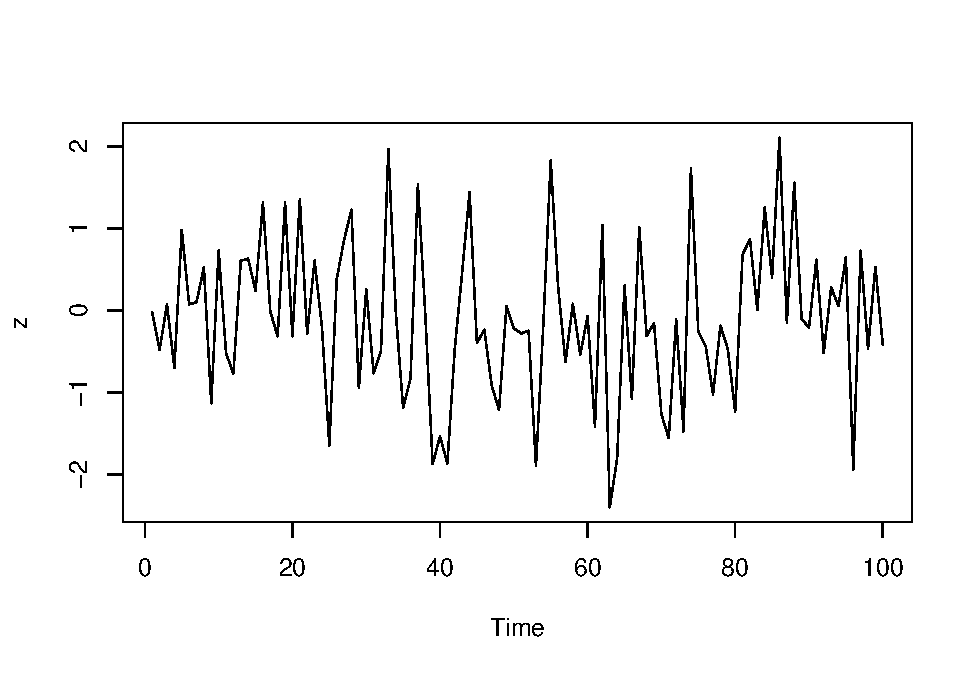
\includegraphics{_main_files/figure-latex/exposition-1.pdf}

\hypertarget{estilo-de-programauxe7uxe3o}{%
\section{Estilo de programação}\label{estilo-de-programauxe7uxe3o}}

Recomendações do próprio Hadley Wickham no livro: \href{https://style.tidyverse.org/pipes.html}{The tidyverse style guide}

Um bom estilo de programação é comparável a uma pontuação correta: você pode
entender o texto sem ela,
noentantoelatornaascoisasmuitosmaisfáceisdeseremlidas.

Todos os guias de estilo são fudamentalmente opinativos. Algumas decisões
tornam programar genuinamente mais fácil (especialmente quando correspondemos
recuos com a estrutura), mas muitas decisões são arbitrárias. O mais importante
em um guideline de estilo é que ele fornece consistência, tornando a
programação mais fácil de escrever porque você precisa tomar menos decisões.

Dois pacotes de R suportam esse estilo:

\begin{itemize}
\item
  \href{http://styler.r-lib.org}{styler} permite que você corrija
  interativamente o estilo de um texto selecionado, arquivos, ou projetos
  inteiros. Ele inclui um add-in no RStudio, a forma mais fácil de
  re-estilizar um código existente.

  \begin{center}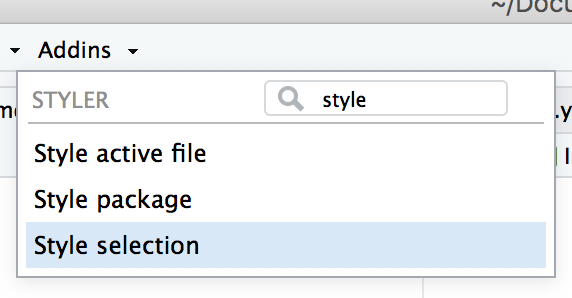
\includegraphics[width=2.6in]{figuras/styler-addin} \end{center}
\item
  \href{https://github.com/jimhester/lintr}{lintr} realiza checagens
  automáticas para confirmar que o seu código está conforme o estilo.
\end{itemize}

\hypertarget{pipes-e-estilo-de-programauxe7uxe3o}{%
\subsection{Pipes e estilo de programação}\label{pipes-e-estilo-de-programauxe7uxe3o}}

Utilize \texttt{\%\textgreater{}\%} para enfatizar a sequência de ações, em vez do objeto nos quais estão sendo realizadas.

Evite utilizar o pipe quando:

\begin{itemize}
\item
  Você precisa manipular mais de um objeto ao mesmo tempo. Limite a utilização de pipes para uma sequência de etapas aplicadas a um objeto primário.
\item
  Existem objetos intermediários significativos que podem ser dados nomes informativos.
\end{itemize}

\hypertarget{espauxe7o-em-branco}{%
\subsubsection{Espaço em branco}\label{espauxe7o-em-branco}}

\texttt{\%\textgreater{}\%} deve ser sempre precedido de um espaço em branco, e sempre sucedido por uma nova linha.

Após a primeira etapa, cada linha deve ser indexada por dois espaços. Essa estrutura torna mais fácil a adição de novas etapas (ou rearranjar etapas existentes) e torna mais difícil de ignorar uma etapa.

\begin{Shaded}
\begin{Highlighting}[]
\CommentTok{\# Bom}
\NormalTok{iris }\SpecialCharTok{\%\textgreater{}\%}
  \FunctionTok{group\_by}\NormalTok{(Species) }\SpecialCharTok{\%\textgreater{}\%}
  \FunctionTok{summarize\_if}\NormalTok{(is.numeric, mean) }\SpecialCharTok{\%\textgreater{}\%}
  \FunctionTok{ungroup}\NormalTok{() }\SpecialCharTok{\%\textgreater{}\%}
  \FunctionTok{gather}\NormalTok{(measure, value, }\SpecialCharTok{{-}}\NormalTok{Species) }\SpecialCharTok{\%\textgreater{}\%}
  \FunctionTok{arrange}\NormalTok{(value)}

\CommentTok{\# Ruim}
\NormalTok{iris }\SpecialCharTok{\%\textgreater{}\%} \FunctionTok{group\_by}\NormalTok{(Species) }\SpecialCharTok{\%\textgreater{}\%} \FunctionTok{summarize\_all}\NormalTok{(mean) }\SpecialCharTok{\%\textgreater{}\%}
\NormalTok{ungroup }\SpecialCharTok{\%\textgreater{}\%} \FunctionTok{gather}\NormalTok{(measure, value, }\SpecialCharTok{{-}}\NormalTok{Species) }\SpecialCharTok{\%\textgreater{}\%}
\FunctionTok{arrange}\NormalTok{(value)}
\end{Highlighting}
\end{Shaded}

\hypertarget{linhas-muito-longas}{%
\subsubsection{Linhas muito longas}\label{linhas-muito-longas}}

Se os argumentos de uma função não cabem em uma linha, coloque cada argumento
em sua própria linha e recue:

\begin{Shaded}
\begin{Highlighting}[]
\NormalTok{iris }\SpecialCharTok{\%\textgreater{}\%}
  \FunctionTok{group\_by}\NormalTok{(Species) }\SpecialCharTok{\%\textgreater{}\%}
  \FunctionTok{summarise}\NormalTok{(}
    \AttributeTok{Sepal.Length =} \FunctionTok{mean}\NormalTok{(Sepal.Length),}
    \AttributeTok{Sepal.Width =} \FunctionTok{mean}\NormalTok{(Sepal.Width),}
    \AttributeTok{Species =} \FunctionTok{n\_distinct}\NormalTok{(Species)}
\NormalTok{  )}
\end{Highlighting}
\end{Shaded}

\hypertarget{pipes-curtos}{%
\subsubsection{Pipes curtos}\label{pipes-curtos}}

Um pipe de apenas uma etapa pode permanecer em uma linha, mas a não ser que
você pretenda expandir ele posteriormente, você deve considerar reescrever seu
código como uma função.

\begin{Shaded}
\begin{Highlighting}[]
\CommentTok{\# Bom}
\NormalTok{iris }\SpecialCharTok{\%\textgreater{}\%} \FunctionTok{arrange}\NormalTok{(Species)}

\NormalTok{iris }\SpecialCharTok{\%\textgreater{}\%} 
  \FunctionTok{arrange}\NormalTok{(Species)}

\FunctionTok{arrange}\NormalTok{(iris, Species)}
\end{Highlighting}
\end{Shaded}

Às vezes é útil incluir um pipe curto como um argumento de uma função em um
pipe maior. Considere cuidadosamente se o código é mais legível com um pipe
curto de uma linha ou se é melhor mover o código para fora do pipe e dar um
nome evocativo.

\begin{Shaded}
\begin{Highlighting}[]
\CommentTok{\# Bom}
\NormalTok{x }\SpecialCharTok{\%\textgreater{}\%}
  \FunctionTok{select}\NormalTok{(a, b, w) }\SpecialCharTok{\%\textgreater{}\%}
  \FunctionTok{left\_join}\NormalTok{(y }\SpecialCharTok{\%\textgreater{}\%} \FunctionTok{select}\NormalTok{(a, b, v), }\AttributeTok{by =} \FunctionTok{c}\NormalTok{(}\StringTok{"a"}\NormalTok{, }\StringTok{"b"}\NormalTok{))}

\CommentTok{\# Melhor}
\NormalTok{x\_join }\OtherTok{\textless{}{-}}\NormalTok{ x }\SpecialCharTok{\%\textgreater{}\%} \FunctionTok{select}\NormalTok{(a, b, w)}
\NormalTok{y\_join }\OtherTok{\textless{}{-}}\NormalTok{ y }\SpecialCharTok{\%\textgreater{}\%} \FunctionTok{select}\NormalTok{(a, b, v)}
\FunctionTok{left\_join}\NormalTok{(x\_join, y\_join, }\AttributeTok{by =} \FunctionTok{c}\NormalTok{(}\StringTok{"a"}\NormalTok{, }\StringTok{"b"}\NormalTok{))}
\end{Highlighting}
\end{Shaded}

\hypertarget{nenhum-argumento}{%
\subsubsection{Nenhum argumento}\label{nenhum-argumento}}

magrittr permite a omissão dos \texttt{()} em funções que não têm argumentos. Evite
isso.

\begin{Shaded}
\begin{Highlighting}[]
\CommentTok{\# Bom}
\NormalTok{x }\SpecialCharTok{\%\textgreater{}\%} 
  \FunctionTok{unique}\NormalTok{() }\SpecialCharTok{\%\textgreater{}\%}
  \FunctionTok{sort}\NormalTok{()}

\CommentTok{\# Ruim}
\NormalTok{x }\SpecialCharTok{\%\textgreater{}\%} 
\NormalTok{  unique }\SpecialCharTok{\%\textgreater{}\%}
\NormalTok{  sort}
\end{Highlighting}
\end{Shaded}

\hypertarget{atribuiuxe7uxe3o}{%
\subsection{Atribuição}\label{atribuiuxe7uxe3o}}

Existem três tipos aceitáveis de atribuição:

\begin{itemize}
\item
  Nome da variável e atribuição em linhas separadas:

\begin{Shaded}
\begin{Highlighting}[]
\NormalTok{iris\_long }\OtherTok{\textless{}{-}}
\NormalTok{  iris }\SpecialCharTok{\%\textgreater{}\%}
  \FunctionTok{gather}\NormalTok{(measure, value, }\SpecialCharTok{{-}}\NormalTok{Species) }\SpecialCharTok{\%\textgreater{}\%}
  \FunctionTok{arrange}\NormalTok{(}\SpecialCharTok{{-}}\NormalTok{value)}
\end{Highlighting}
\end{Shaded}
\item
  Nome da variável e atribuição na mesma linha:

\begin{Shaded}
\begin{Highlighting}[]
\NormalTok{iris\_long }\OtherTok{\textless{}{-}}\NormalTok{ iris }\SpecialCharTok{\%\textgreater{}\%}
  \FunctionTok{gather}\NormalTok{(measure, value, }\SpecialCharTok{{-}}\NormalTok{Species) }\SpecialCharTok{\%\textgreater{}\%}
  \FunctionTok{arrange}\NormalTok{(}\SpecialCharTok{{-}}\NormalTok{value)}
\end{Highlighting}
\end{Shaded}
\item
  Atribuição no final do pipe com \texttt{-\textgreater{}}:

\begin{Shaded}
\begin{Highlighting}[]
\NormalTok{iris }\SpecialCharTok{\%\textgreater{}\%}
  \FunctionTok{gather}\NormalTok{(measure, value, }\SpecialCharTok{{-}}\NormalTok{Species) }\SpecialCharTok{\%\textgreater{}\%}
  \FunctionTok{arrange}\NormalTok{(}\SpecialCharTok{{-}}\NormalTok{value) }\OtherTok{{-}\textgreater{}}
\NormalTok{  iris\_long}
\end{Highlighting}
\end{Shaded}

  Talvez seja a maneira mais natural de escrever, mas torna a
  leitura mais difícil: quando o nome vem primeiro ele age como um
  cabeçalho para lembrar o propósito do pipe.
\end{itemize}

O pacote magrittr fornece o operador \texttt{\%\textless{}\textgreater{}\%} como um atalho para modificar um objeto. Evite esse operador.

\begin{Shaded}
\begin{Highlighting}[]
\CommentTok{\# Bom}
\NormalTok{x }\OtherTok{\textless{}{-}}\NormalTok{ x }\SpecialCharTok{\%\textgreater{}\%} 
  \FunctionTok{abs}\NormalTok{() }\SpecialCharTok{\%\textgreater{}\%} 
  \FunctionTok{sort}\NormalTok{()}
  
\CommentTok{\# Ruim}
\NormalTok{x }\SpecialCharTok{\%\textless{}\textgreater{}\%}
  \FunctionTok{abs}\NormalTok{() }\SpecialCharTok{\%\textgreater{}\%} 
  \FunctionTok{sort}\NormalTok{()}
\end{Highlighting}
\end{Shaded}

\hypertarget{trabalhando-em-ambiente-de-projetos}{%
\chapter{Trabalhando em ambiente de projetos}\label{trabalhando-em-ambiente-de-projetos}}

Certos aspectos da análise de dados podem não ser tão agradáveis. Por exemplo:

\begin{itemize}
\tightlist
\item
  Manter o controle de todos os arquivos que meu projeto gera.
\item
  Data wrangling (Disputa de dados).
\end{itemize}

\hypertarget{criando-um-projeto-no-r}{%
\section{Criando um projeto no R}\label{criando-um-projeto-no-r}}

Ao trabalhar em um projeto, você provavelmente cria muitos arquivos diferentes para vários propósitos, especialmente R Scripts. Se você não tomar cuidado, esse arquivo será armazenado no local padrão do seu sistema, que pode não estar onde você deseja.

O RStudio permite que você gerencie todo o seu projeto de forma intuitiva e conveniente através dos arquivos do R Project. O uso de arquivos do R Project vem com algumas vantagens, por exemplo:

\begin{itemize}
\item
  Todos os arquivos que você gera estão no mesmo lugar. Seus dados, seus códigos, seus plots (gráficos), seus relatórios, etc., estão todos juntos em um só lugar sem que você precise gerenciar os arquivos manualmente. Isso se deve ao fato de o RStudio definir o diretório raiz para a pasta em que seu projeto foi salvo.
\item
  Se você deseja compartilhar seu projeto, pode compartilhar a pasta inteira e outras pessoas podem reproduzir rapidamente sua pesquisa ou ajudar a corrigir problemas. Isso ocorre porque todos os caminhos de arquivo são relativos e não absolutos.
\item
  Você pode, mais facilmente, usar o GitHub para backups e o chamado `controle de versão', que permite rastrear as alterações feitas em seu código ao longo do tempo.
\end{itemize}

Por enquanto, o motivo mais importante para usar os arquivos do R Project é a conveniência da organização dos arquivos e a capacidade de compartilhá-los facilmente com colegas.

Para criar um projeto no R:

\begin{enumerate}
\def\labelenumi{\arabic{enumi}.}
\item
  Selecione \texttt{File\ \textgreater{}\ New\ Project} da barra de menu.
\item
  Selecione \texttt{New\ Directory} da janela pop-up.
\end{enumerate}

\begin{center}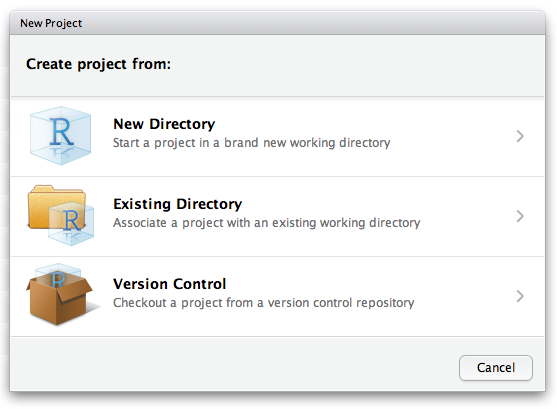
\includegraphics[width=2.53in]{figuras/projects_new} \end{center}

\begin{enumerate}
\def\labelenumi{\arabic{enumi}.}
\setcounter{enumi}{2}
\tightlist
\item
  Selecione \texttt{Novo\ Projeto}.
\end{enumerate}

\hypertarget{organizando-seu-projeto}{%
\section{Organizando seu projeto}\label{organizando-seu-projeto}}

Esta seção não está diretamente relacionada ao RStudio, R ou análise de dados em geral. Em vez disso, quero transmitir a você que uma boa estrutura de pastas pode percorrer um longo caminho.

É um excelente hábito começar a pensar em estruturas de pastas antes de começar a trabalhar em seu projeto. Colocar seus arquivos em pastas dedicadas, em vez de mantê-los soltos em um contêiner, acelerará seu trabalho e evitará a frustração de não encontrar os arquivos necessários. Eu tenho um modelo que uso regularmente. Você pode criá-lo do zero no RStudio ou abrir seu navegador de arquivos e criar as pastas lá. O RStudio não se importa com a maneira como você faz isso. Se você quiser gastar menos tempo configurando isso, você pode usar a função create\_project\_folder() do pacote r4np. Ele cria todas as pastas conforme mostrado na figura abaixo:

Você provavelmente notou que minhas pastas têm números na frente delas. Faço isso para garantir que todas as pastas estejam na ordem que desejo, que geralmente não é a ordem alfabética que meu computador sugere. Eu uso dois dígitos porque posso ter mais de nove pastas para um projeto, e a pasta dez seria listada como a terceira pasta nesta lista. Com essa estratégia de arquivamento, será fácil encontrar o que eu preciso. Até mesmo outros podem entender facilmente o que armazenei onde. É simplesmente ``arrumado'', semelhante a como queremos que nossos dados sejam.

  \bibliography{book.bib,packages.bib}

\end{document}
